\documentclass[tikz,border=5pt]{standalone}
\usepackage{fourier}
\begin{document}
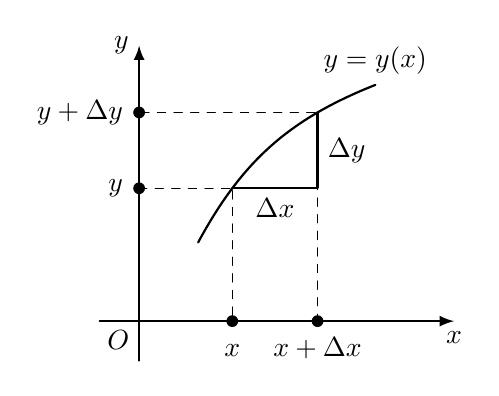
\begin{tikzpicture}[
        mydot/.style={circle,fill,inner sep=1.5pt},
        >=latex,line cap=round,line join=round
    ]
    \draw[thick,->] (0,-.5) -- (0,3.5) coordinate (y) node [left] {$y$};
    \draw[thick,->] (-.5,0) -- (4,0) coordinate (x) node [below] {$x$};
    \draw[thick] 
    (.75,1) to[bend left = 20] 
    node [near start, inner sep = 0pt] (tmpa) {} 
    node [near end, inner sep = 0pt] (tmpb) {}
    (3,3) node[above] {$y=y(x)$};
    \draw[dashed] 
    (tmpa) -- (tmpa -| y) node[mydot,label=left:$y$] {}
    (tmpa) -- (tmpa |- x) node[mydot,label=below:$x\vphantom{\Delta}$] {}
    (tmpb) -- (tmpb -| y) node[mydot,label=left:$y+\Delta y$] {}
    (tmpb) -- (tmpb |- x) node[mydot,label=below:$x+\Delta x$] {}
    (0,0) node[below left] {$O$}
    ;
    \draw[thick] (tmpa.center) -- node[below] {$\Delta x$} (tmpa -| tmpb) -- node[right] {$\Delta y$} (tmpb.center);
\end{tikzpicture}   
\end{document}